\section{Measurement of Thermal Energy}


%Specific Heat Capacity (calorimeter)

\subsection{Specific Heats}
\begin{itemize}
\item{Preparation Time: 5 minutes}
\item{Materials: thermometer, water, any liquid, measuring cylinder, small pot, glass container or jar, heat source}
\item{Procedure: Measure a known volume of the liquid into a glass container. Heat the water in the pot over a jiko or stove until it is significantly warmer than the other liquid. Measure the volume of the water in the measuring cylinder. Before mixing the liquids, measure each temperature and record it. Now pour the hot water into the other liquid and wait for the temperature of the mixture to equalize. When the temperature levels off, measure and record it. With this data, you can calculate the specific heat capacity of the liquid.}
\item{Theory: Specific heat capacity is given by where H is the heat needed to raise a mass m a temperature T. Since the liquid and water are being mixed, the same amount of energy used to raise the liquid’s temperature is lost by the water to cool it down. We can set the heat of water Hw equal to the heat of the liquid Hl. The masses of the substances are known (by using the mole equations), and you measured the changes in temperature with the thermometer. The specific heat capacity of water is 4200 J/kgK, so you can solve for the specific heat capacity of the liquid.}
\end{itemize}


\subsection{Designing a Calorimeter}

\subsubsection*{Learning Objectives}
\begin{itemize}
\item{To create a calorimeter}
\item{To measure specific heat capacity of different materials}
\end{itemize}

\subsubsection*{Background Information}
Materials can be distinguished by their specific heat capacity. Using the relation: Heat = mass x specific heat capacity x change temperature. You can calculate specific heat capacity for liquid objects or solid objects.

\subsubsection*{Materials}
Box made from wood, ceiling board or a piece of wood, aluminum cup, aluminum wire, pieces of blanket or sweater, and a thermometer.

\subsubsection*{Preparation Procedure}
\begin{enumerate}
\item{Use wood to make a box with 10 cm x 10 cm x 12 cm width.}
\item{Prepare a top cover with wood or ceiling materials.}
\item{Use aluminium wire to make a stirrer.}
\item{Prepare a stirrer-holder with an insulator material like rubber.}
\item{Remove the aluminum cup handle.}
\end{enumerate}

\begin{figure}
\begin{center}
%\def\svgwidth{350pt}
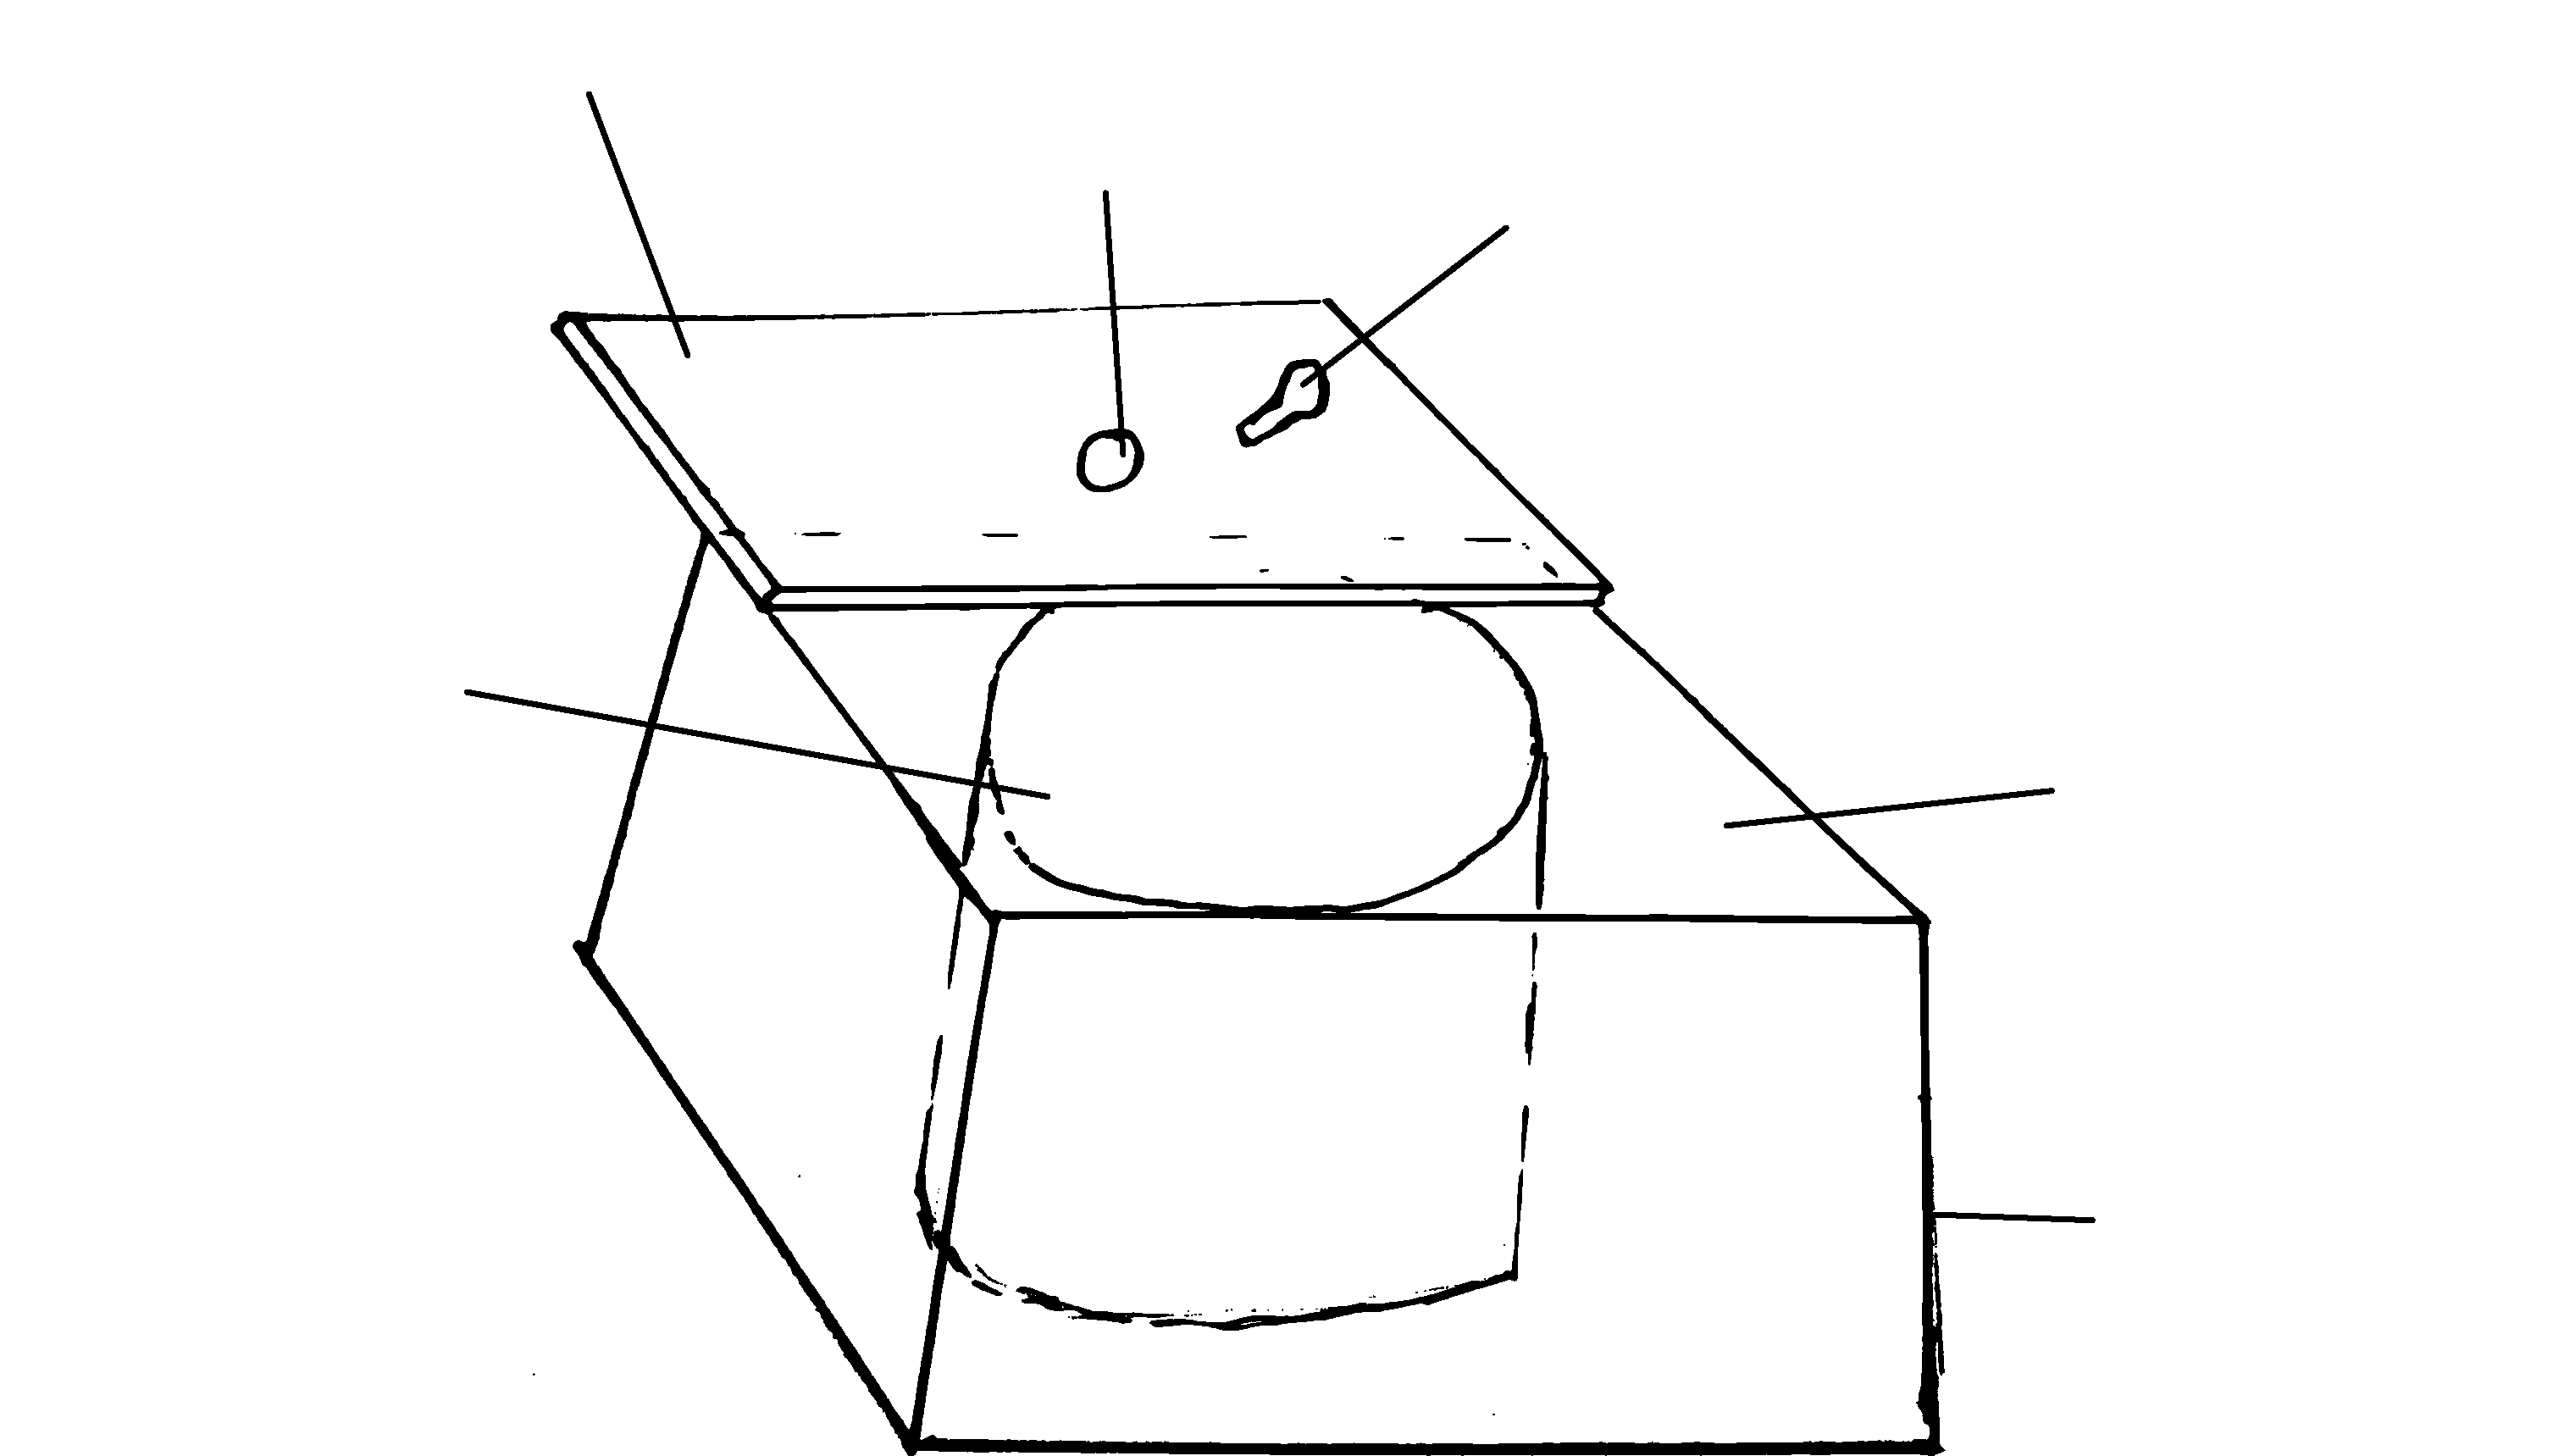
\includegraphics{./img/calorimeter.png}
\caption{Construction of a calorimeter}
\label{fig:calorimeter}
\end{center}
\end{figure}

\subsubsection*{Activity Procedure}
\begin{enumerate}
\item{Place the piece of blanket in the box.}
\item{Put the aluminum cup in the box.}
\item{Put stirrer in the aluminium cup.}
\item{Place the top cover on the box.}
\item{Place the stirrer holder.}
\item{Insert the thermometer in the middle hole.}
\end{enumerate}

\subsubsection*{Results and Conclusions}
Calorimeter can be used to determine the specific capacity of liquid and solid objects.

\subsubsection*{Discussion Questions}
\begin{enumerate}
\item{Why is it important for the calorimeter and stirrer to be made of the same material.}
\item{Discuss an experiment that requires a calorimeter?}
\end{enumerate}

\subsubsection*{Notes}
Heat energy transfer depends on the material. Different materials transfer heat differently. The specific heat capacity can be obtain by finding heat transfer from one material to another. By using a calorimeter 
you can find the specific heat capacity of the material. The specific heat capacity tell the ability of material to loose or gain heat energy.


%Change of State

\subsection{Boiling Water at Room Temperature}

\subsubsection*{Learning Objectives}
\begin{itemize}
\item{To observe the effect of pressure on the boiling point of water} 
\item{To explain why the boiling point of water decreases with pressure} 
\end{itemize}

\subsubsection*{Background Information}
Boiling and melting points are usually assumed to be constant. For example, the melting point of ice is 0-degrees C and the boiling point is 100-degrees C. However, this is only true at STP, or Standard Temperature and Pressure. Standard pressure is 760 mm Hg, which is only true at sea level. Pressure decreases with elevation, therefore the boiling point of water also decreases. The boiling point of water at sea level will be measurably different from the boiling point on a mountain.  

\subsubsection*{Materials}
10 mL or 20 mL syringe without needle, water

\subsubsection*{Preparation Procedure}
Collect the syringe and remove the needle.

\subsubsection*{Activity Procedure}
\begin{enumerate}
\item{Fill the syringe with a small amount of water.} 
\item{Place your thumb over the opening of the syringe.} 
\item{Pull the plunger out as far as you can.} 
\item{Observe the behavior of the water in the syringe.} 
\end{enumerate}

\begin{figure}
\begin{center}
%\def\svgwidth{150pt}
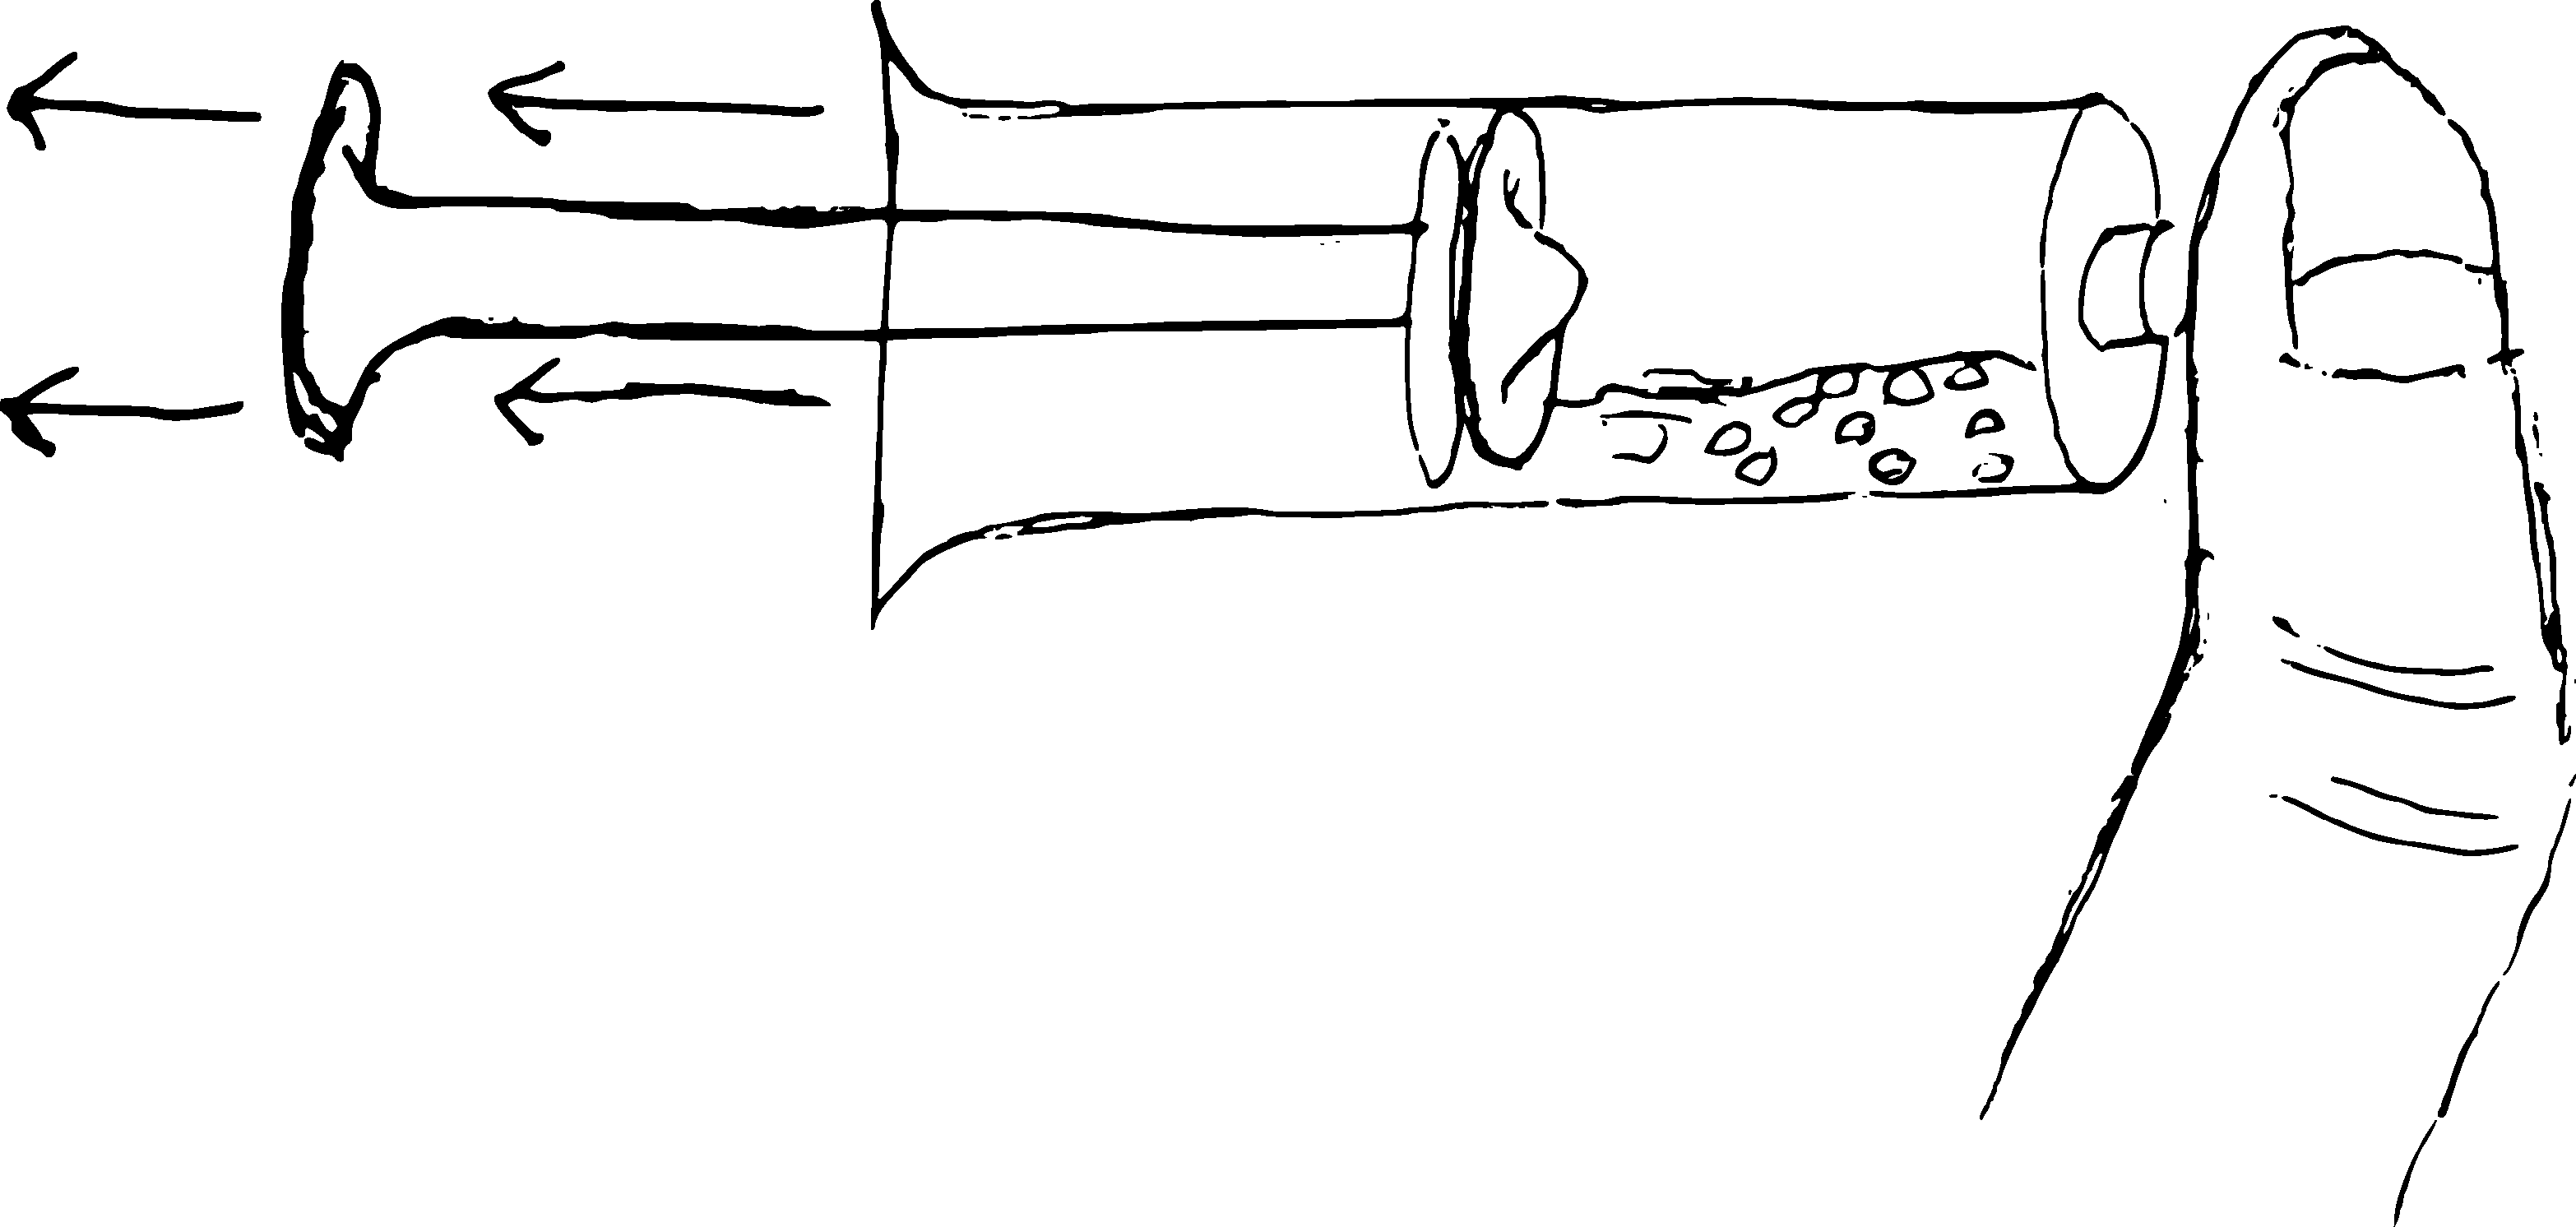
\includegraphics{./img/boiling-room-temp.png}
\caption{Boiling Water at Room Temperature}
\label{fig:boiling-room-temp}
\end{center}
\end{figure}

\subsubsection*{Results and Conclusions}
When the plunger is pulled out as far as it will go (without removing it from the syringe), the water will begin to bubble, meaning that it is boiling. This is because the pressure inside the syringe is decreasing, and the boiling point of the water is decreasing with the pressure. When the boiling point is reduced to room temperature, the water begins to boil.  

\subsubsection*{Clean Up Procedure}
Dispose of the water and return all materials to their proper places.

\subsubsection*{Discussion Questions}
\begin{enumerate}
\item{Why is it difficult to pull the plunger out when your thumb is covering the syringe opening?}
\item{By pulling out the plunger, are you increasing or decreasing the pressure in the syringe?}
\item{What happens to the water when you pull the plunger as far as you can?}
\end{enumerate}

\subsubsection*{Notes}
When pulling water into the syringe, you only need to take a small amount. If you take too much water, you will not be able to reduce the pressure in the syringe before the plunger comes out.  
Before doing this activity, be sure that the students understand that the presence of bubbles means that a liquid is boiling.


\subsection{Latent Heat of Fusion} % or heat capacity???

\subsubsection*{Learning Objectives}
\begin{itemize}
\item{To observe the process of fusion} 
\item{To explain the difference between heat capacity and latent heat} 
\item{To observe the constant temperature of latent heat} 
\end{itemize}

\subsubsection*{Background Information}
As a substance is heated, there are two types off heat involved. Heat capacity is the heat needed to raise the temperature of the substance; latent heat is the heat needed to change the substance from one state to another.  
Heat capacity is the heat that we normally see: you can measure it with a thermometer as it raises the temperature of a body. Latent heat, however, is "hidden.  " This means that latent heat does not raise the temperature of a body, so it cannot be measured with a thermometer.  
When a substance is heated, its temperature increases as it gains heat as per its heat capacity. However, when it changes state from solid to liquid or liquid to gas, its temperature remains constant as it is absorbing latent heat.  

\subsubsection*{Materials}
Heat source, water, small cooking pot, thermometer.

\subsubsection*{Preparation Procedure}
The thermometer may be a real thermometer if you want to measure the temperature at which latent heat is absorbed. However, you can use any liquid in a capillary tube to see the expansion of the liquid. When the latent heat is used and the water is changing state, the liquid in the tube will stop expanding.

\subsubsection*{Activity Procedure}
\begin{enumerate}
\item{Fill the pot about half-way with water.} 
\item{Place the thermometer in the water.} 
\item{Turn on the heat and place the pot over the heat.} 
\item{Observe the rise in temperature as the water is heated. Record the temperature every 10 seconds.} 
\item{Continue recording the temperature every 10 seconds after the water begins to boil.} 
\item{Plot a graph of temperature (vertical axis) against time (horizontal axis).} 
\end{enumerate}

\subsubsection*{Results and Conclusions}
The temperature will be seen to increase steadily as the water is heated. When the water begins to boil, the temperature stops increasing and remains constant while the water vapourizes. The graph will show a steadily increasing temperature until it reaches the boiling point on the vertical axis. This value should be about 100 degrees C. At this point, the temperature will level off as time continues to increase.  

\subsubsection*{Clean Up Procedure}
\begin{enumerate}
\item{Remove the thermometer from the water and pour it out.} 
\item{Turn off the heat and return all materials to their proper places when they are cooled.} 
\end{enumerate}

\subsubsection*{Discussion Questions}
\begin{enumerate}
\item{What happens to the temperature when the water begins to boil?}
\item{What happens to the temperature as the water is heated but before it boils?}
\item{What heat is involved in heating the water?}
\item{What heat is involved in changing the water from a liquid to vapour?}
\end{enumerate}

\subsubsection*{Notes}
It is important to periodically measure the temperature and time as the water heats.  This will allow you to see clearly the boiling point when the latent heat of water becomes a factor.

